
%(BEGIN_QUESTION)
% Copyright 2006, Tony R. Kuphaldt, released under the Creative Commons Attribution License (v 1.0)
% This means you may do almost anything with this work of mine, so long as you give me proper credit

Hydrauliske (væske-) kraftsystemer trenger trykkregulering på samme måte som pneumatiske (luft-)systemer. Trykkstyring må imidlertid gjøres annerledes i et hydraulikksystem. I et pneumatisk system startes og stoppes elmotoren som driver kompressoren for å holde systemtrykket mellom to settpunkter. I et hydraulikksystem går elmotoren som driver fortrengningspumpen kontinuerlig, mens en trykkavlastningsventil regulerer linjetrykket:

$$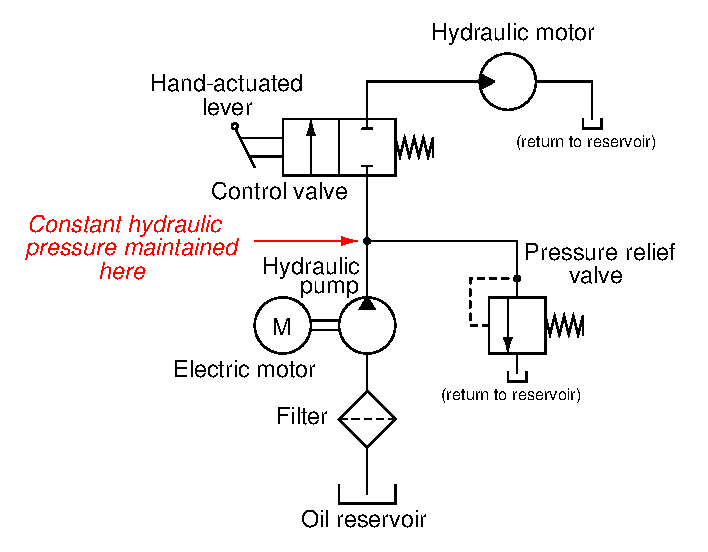
\includegraphics[width=15.5cm]{i00752x01.eps}$$

Uten trykkavlastningsventilen ville hydraulikkpumpen «låst seg» og nektet å rotere når reguleringsventilen sto i «stopp»-stilling (som vist i figuren). Med trykkavlastningsventilen på plass vil pumpen fortsette å rotere, og hydraulikktrykket opprettholdes.

\vskip 10pt

Forklar hvorfor en fortrengnings-hydraulikkpumpe vil «låse seg» hvis utløpslinjen blokkeres, og forklar virkemåten til trykkavlastningsventilen.

\vskip 20pt \vbox{\hrule \hbox{\strut \vrule{} {\bf Forslag til sokratisk diskusjon} \vrule} \hrule}

\begin{itemize}
\item{} Angi hva som måtte vært endret i dette fluidkraftsystemet for å {\it reversere} motorens retning.
\item{} Ville systemet fungert tilfredsstillende dersom trykkavlastningsventilen ble flyttet «nedstrøms» for spolventilen?
\item{} Hvis filteret tetter helt og stopper all strømning gjennom det, ville hydraulikkpumpen da «låse seg» på samme måte som ved blokkert utløpsport?
\item{} Energibevaringsloven sier at energi ikke kan skapes eller ødelegges, men må gjøres rede for i ethvert system. Når spolventilen står i «av»-stilling og motoren ikke beveger seg, hvor blir energien av som pumpen tilfører fluidsystemet? Hvis hydraulikkpumpen for eksempel drives av en 1 hk-motor, hva skjer med all denne effekten når den ikke går til mekanisk arbeid i motoren?
\end{itemize}

\underbar{file i00752}
%(END_QUESTION)





%(BEGIN_ANSWER)

Et helt sentralt begrep her er {\it inkompressibilitet}. Luft er et kompressibelt fluid, mens hydraulikkolje for alle praktiske formål er inkompressibel. Derfor vil en fortrengningspumpe låse seg dersom det inkompressible fluidet ikke har noe sted å strømme ut.

%(END_ANSWER)





%(BEGIN_NOTES)

Formålet med trykkavlastningsventilen er å åpne når trykket når settpunktet, og dermed regulere trykket ved å sende en kontrollert strøm av hydraulikkolje tilbake til reservoaret.

%INDEX% Mekanikk, fluidkraftsystemer: trykkstyring i hydraulikksystem

%(END_NOTES)


